\pagestyle{n-1}
\label{n-1}

\begin{textblock*}{5.625in}(0pt,0pt)%
\vspace*{-3.2cm}
\hspace*{-1.95cm}\includegraphics*[width=160mm]{./imgs/N-1.png}
\end{textblock*}

\pagebreak %RIOT PUSSY

\begin{center}
\hspace*{.5cm}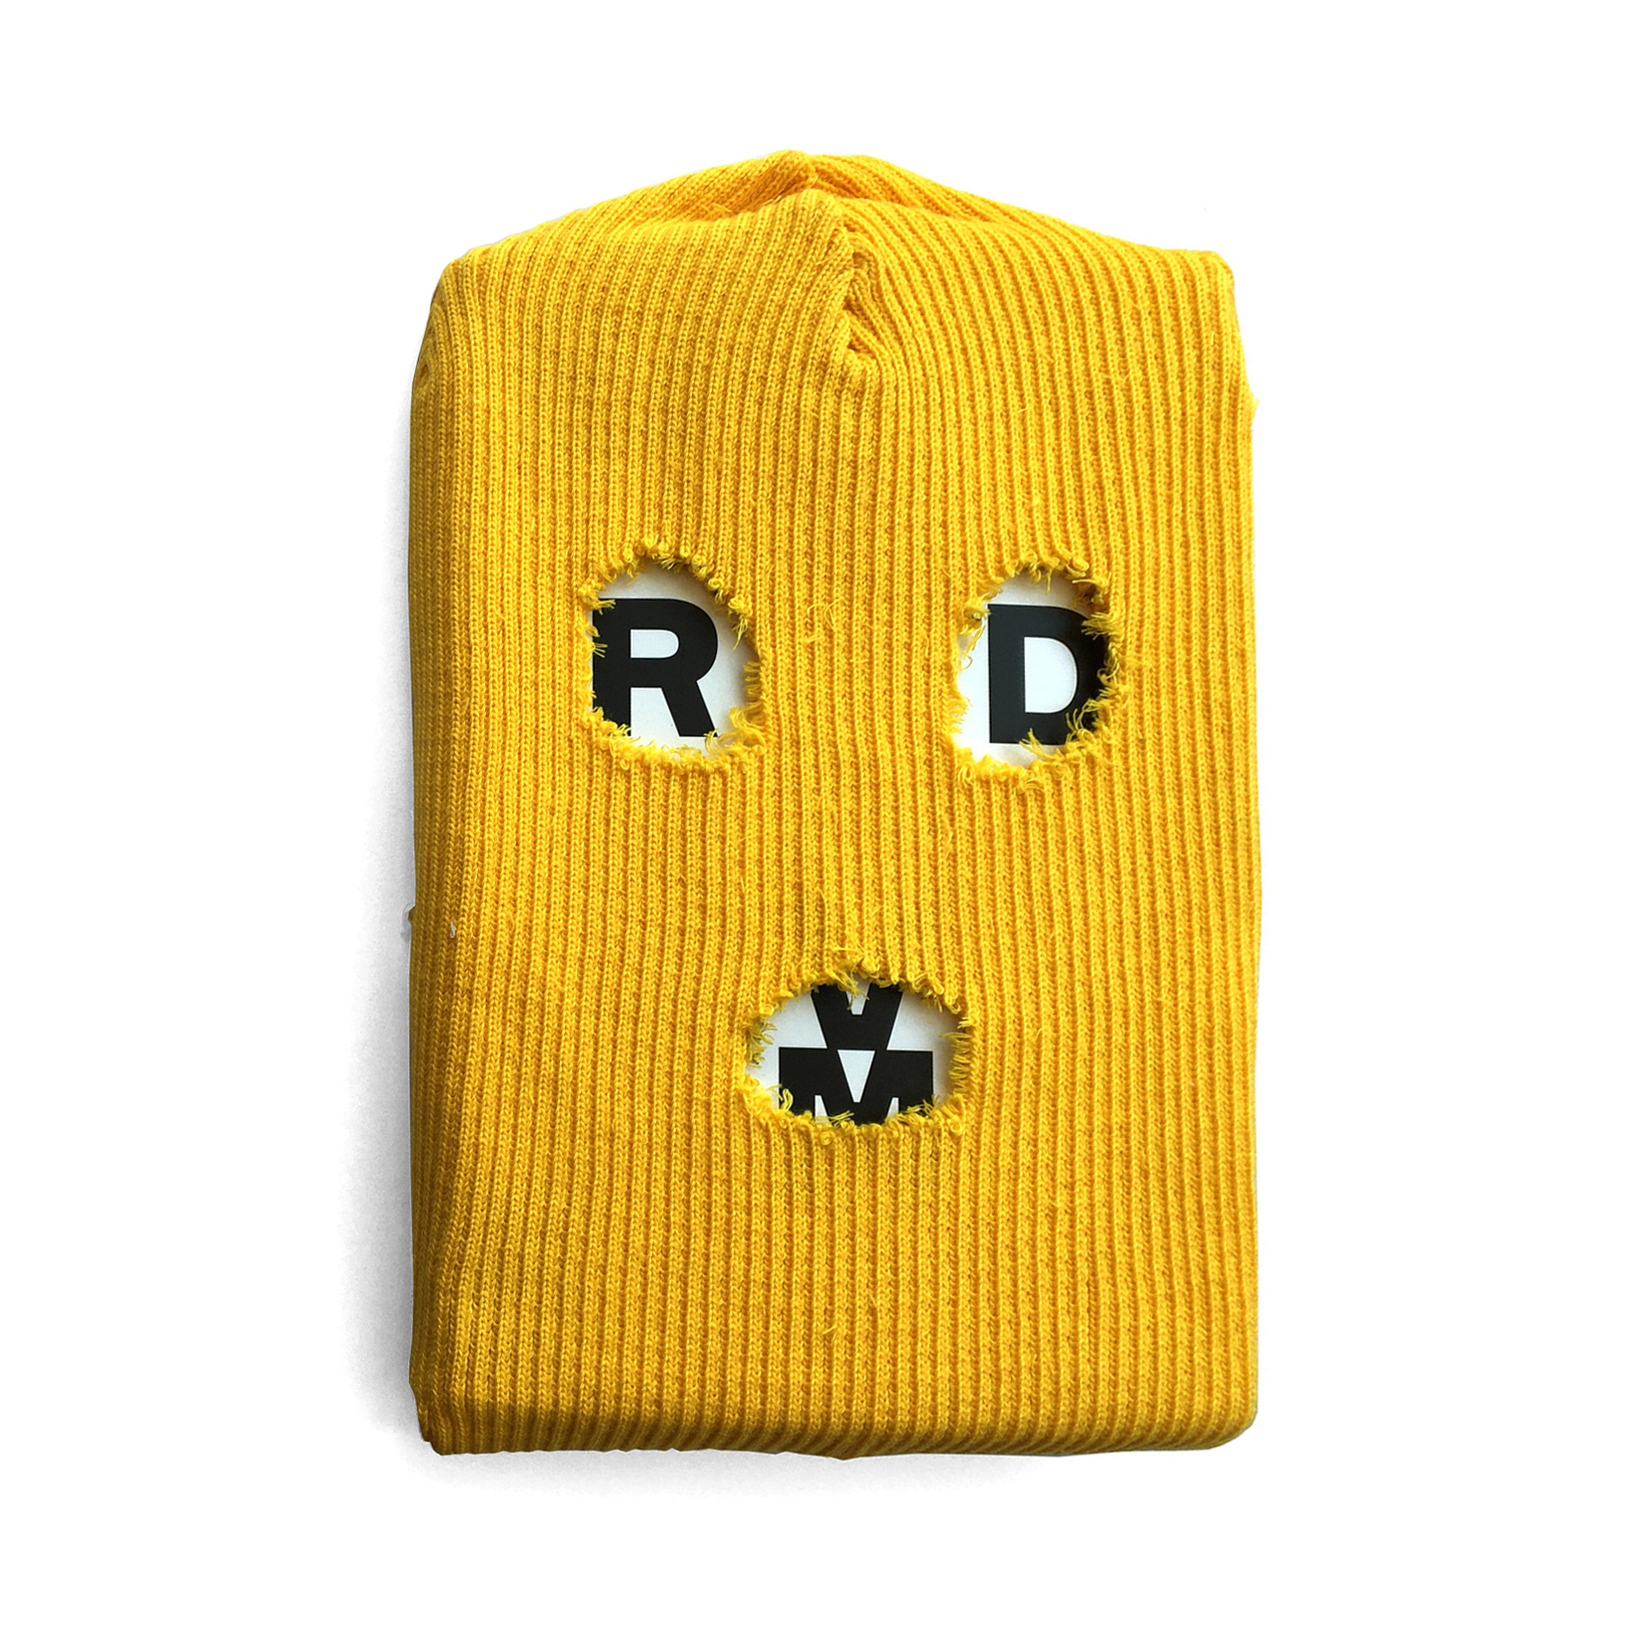
\includegraphics[width=78mm]{./grid/riot.jpg}
\end{center}

\hspace*{-7cm}\hrulefill\hspace*{-7cm}

\medskip

\noindent{}{\slsc{Nós somos Pussy Riot}} é um combo e também um libelo que se interpõe entre o patriarcado capitalista e encarcerador e as mulheres que ele vitimiza, de mais de uma forma: seu conteúdo é revolucionário, mas também o são as várias etapas de seu processo produtivo.

Ele é composto por {\slsc{Riot days}}, um relato cru, alucinatório e apaixonado sobre a prisão e julgamento de Maria Alyokhina em uma colônia penal nos Urais após participar junto com Pussy Riot, sua banda punk feminista, de um protesto punk contra Putin em uma igreja ortodoxa.
E também de dois cordéis --- {\slsc{Sobre (Viver)}} e {\slsc{Engaiolaram"-nos}} --- tudo embalado em balaclavas coloridas, símbolo universal de resistência e luta social, confeccionadas especialmente pela Cooperativa Libertas, de mulheres egressas da máquina do sistema penitenciário brasileiro. Entre a banda Pussy Riot, perseguida em uma Rússia onde direitos das minorias são tolhidos, e as brasileiras que sofrem em um sistema desumano, há muito em comum. 

\vfill

\hspace*{-.4cm}\begin{minipage}[c]{.5\linewidth}
\small{
{\Formular{\textbf{
\hspace*{-.1cm}Título: Nós somos Pussy Riot\\
Autor: Maria Alyokhina\\ 
ISBN: 978-65-8109-713-4\\
Páginas: 216\\
Formato: 14x21cm\\
Preço: R\$ 89,90\\
Editora: n-1 \& Hedra\\
Disponibilidade: Disponível
}}}}
\end{minipage}

\pagebreak %CORPOS QUE IMPORTAM, JUDITH BUTLER


\begin{center}
\hspace*{-3.5cm}\raisebox{5.4cm}{\rotatebox[origin=t]{90}{\huge\Formular{\textbf{Lançamento}}}}
\hspace*{3cm}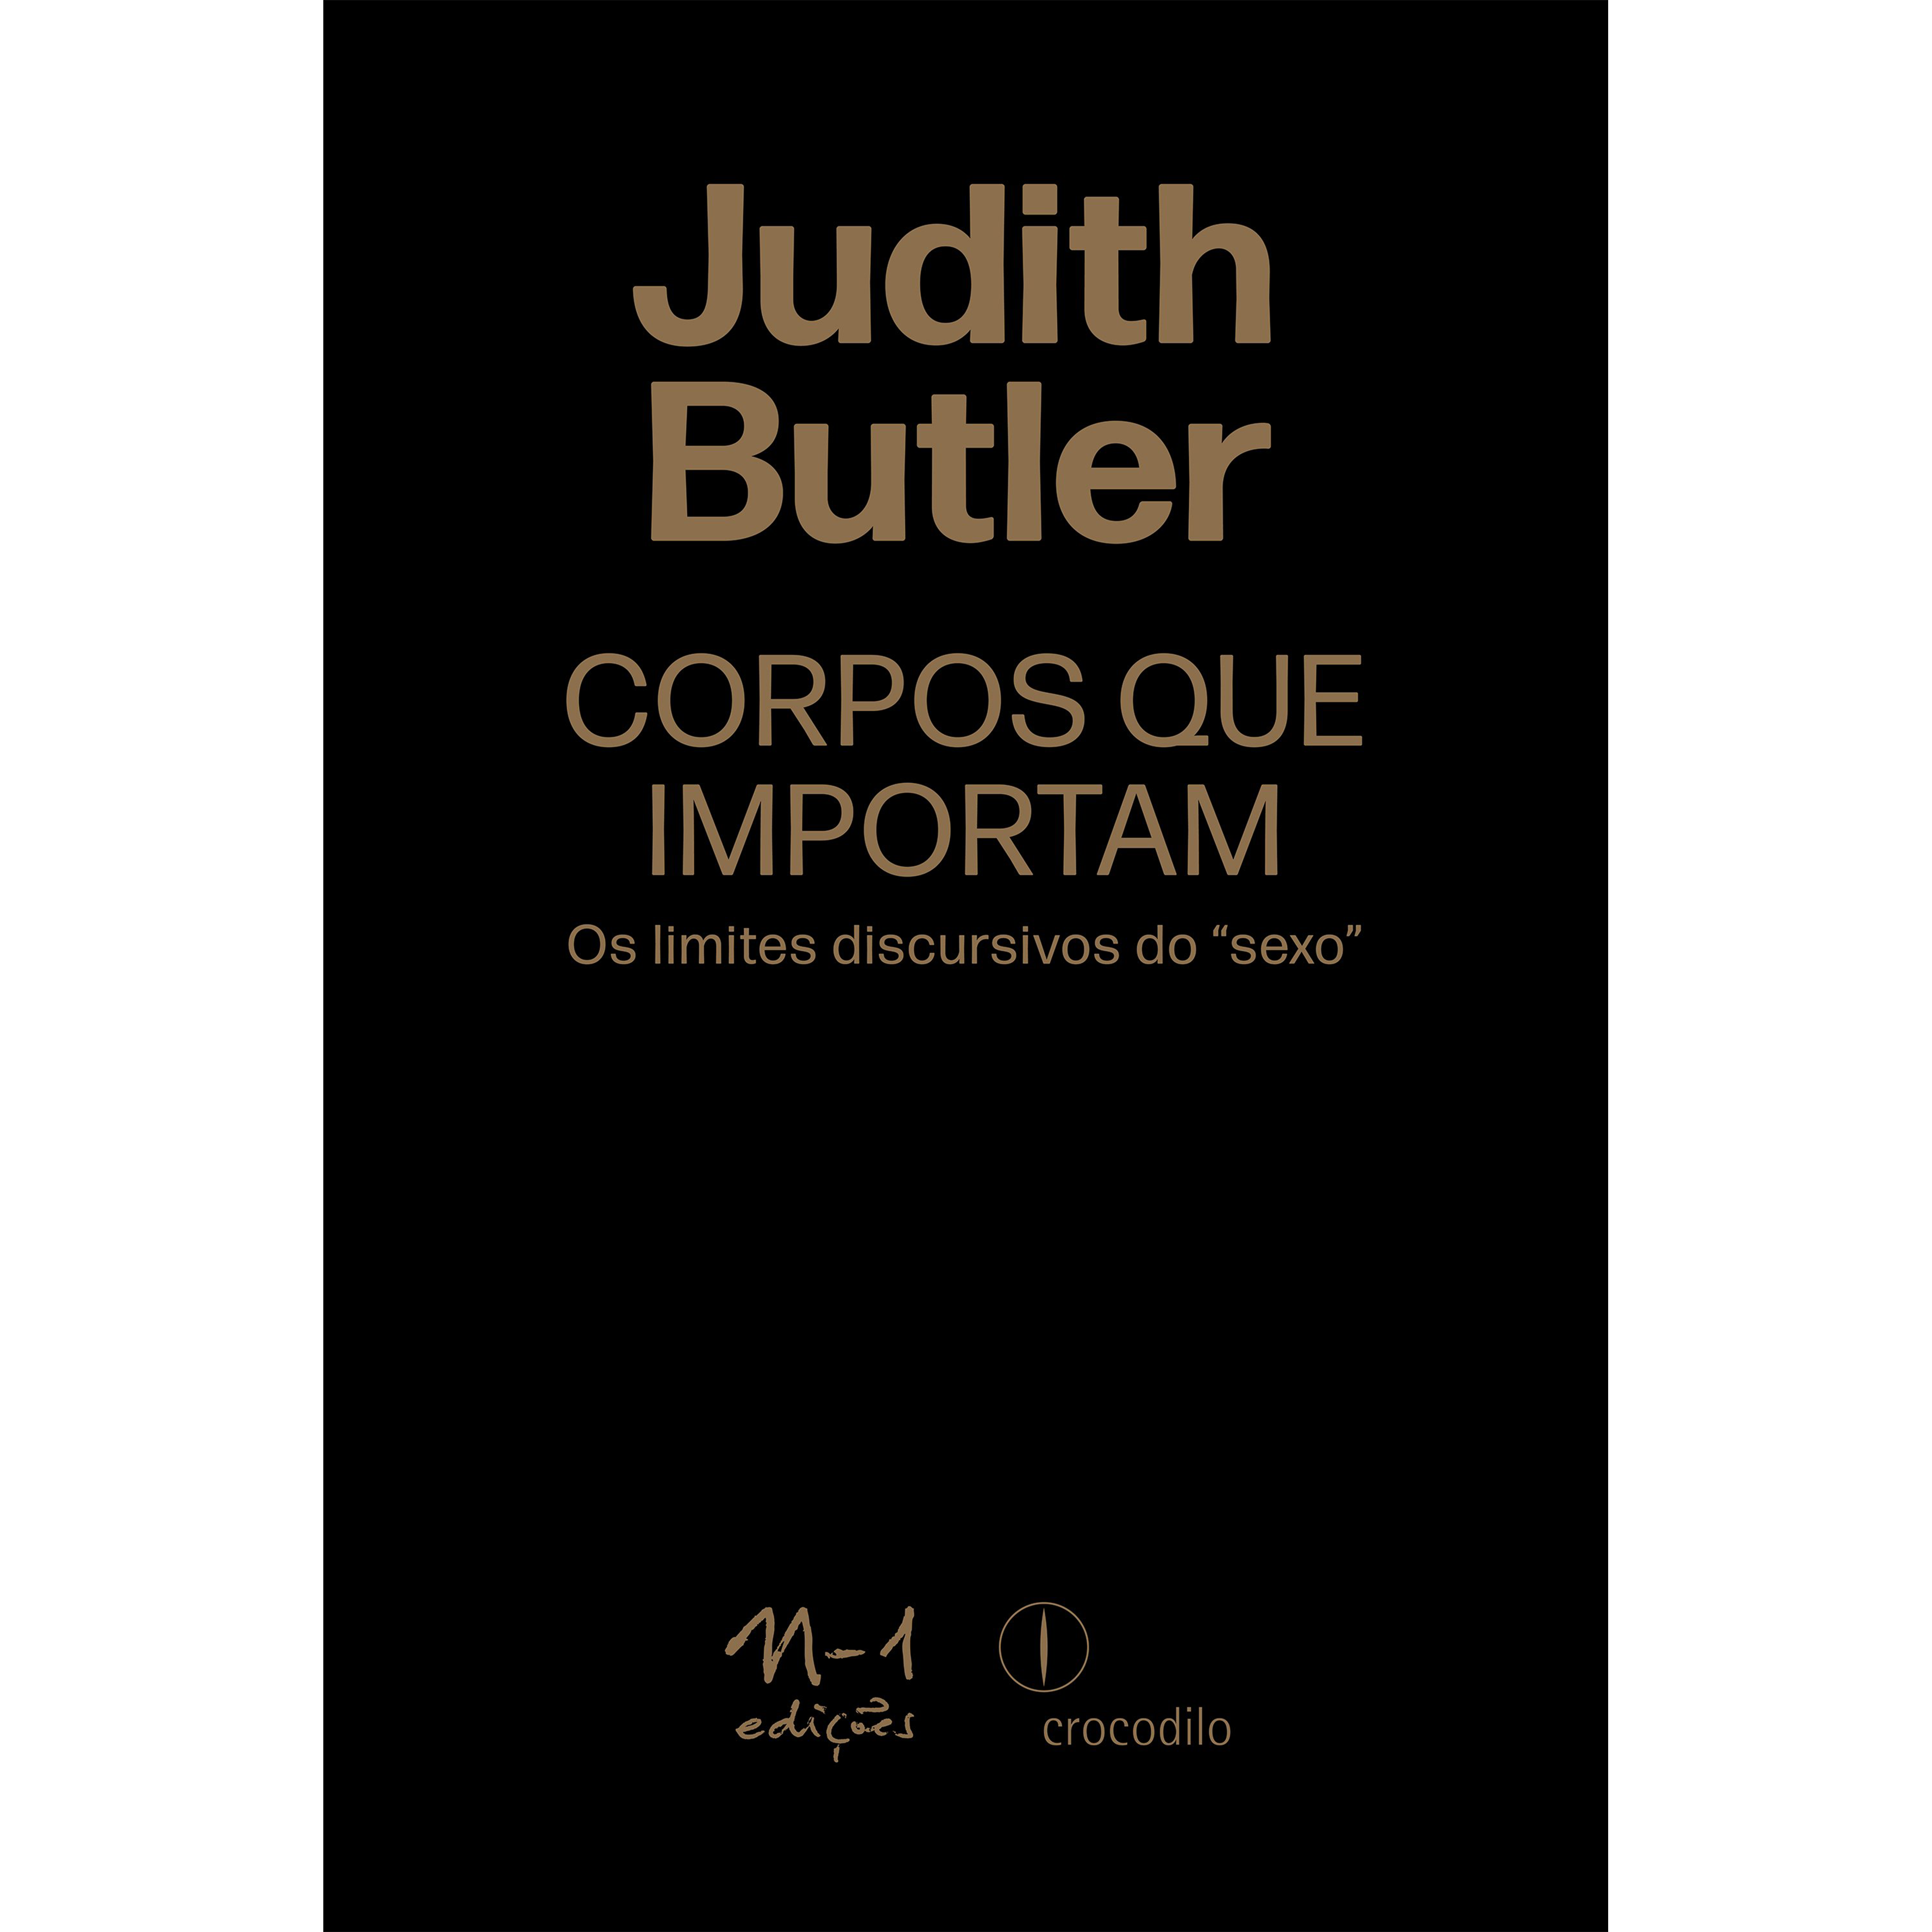
\includegraphics[width=78mm]{./grid/butler.png}
\end{center}

\hspace*{-7cm}\hrulefill\hspace*{-7cm}

\medskip

\noindent{}{\slsc{Corpos que importam}} é sobre pensar a hegemonia heterossexual na criação de matérias [{\slsc{matter}}] sexuais e políticas. Quais são as limitações pelas quais corpos são materializados como “sexuados”? E como devemos entender a “questão” [{\slsc{matter}}] do sexo e dos corpos de modo mais geral, como a circunscrição repetida e violenta da inteligibilidade cultural? Quais corpos importarão [{\slsc{matter}}] --- e por quê?

Nas palavras da filósofa pós"-estruturalista Judith Butler: “Ofereço este texto em parte como forma de reconsiderar algumas seções de meu livro {\slsc{Problemas de gênero}} que causaram confusão, mas também como um esforço para pensar mais sobre o funcionamento da hegemonia heterossexual na criação de matérias [{\slsc{matter}}] sexuais e políticas. Como uma rearticulação crítica de práticas teóricas, incluindo estudos feministas e {\slsc{queer}}, esta obra não pretende ser programática. E ainda como tentativa de esclarecer minhas “intenções”, ela também parece destinada a produzir novos conjuntos de mal"-entendidos. Espero que, ao menos, eles se provem produtivos.”


\vfill

\hspace*{-.4cm}\begin{minipage}[c]{1\linewidth}
\small{
{\Formular{\textbf{
\hspace*{-.1cm}Título: Corpos que importam – os limites discursivos do “sexo”\\
Autor: Judith Butler\\ 
ISBN: 978-65-8109-704-2\\
Páginas: 400\\
Formato: 14x21cm\\
Preço: R\$ 98,00\\
Editora: n-1 \& Crocodilo\\
Disponibilidade: Disponível
}}}}
\end{minipage}

\pagebreak %SOMOS NOSSO CÉREBRO?

\begin{center}
\hspace*{.5cm}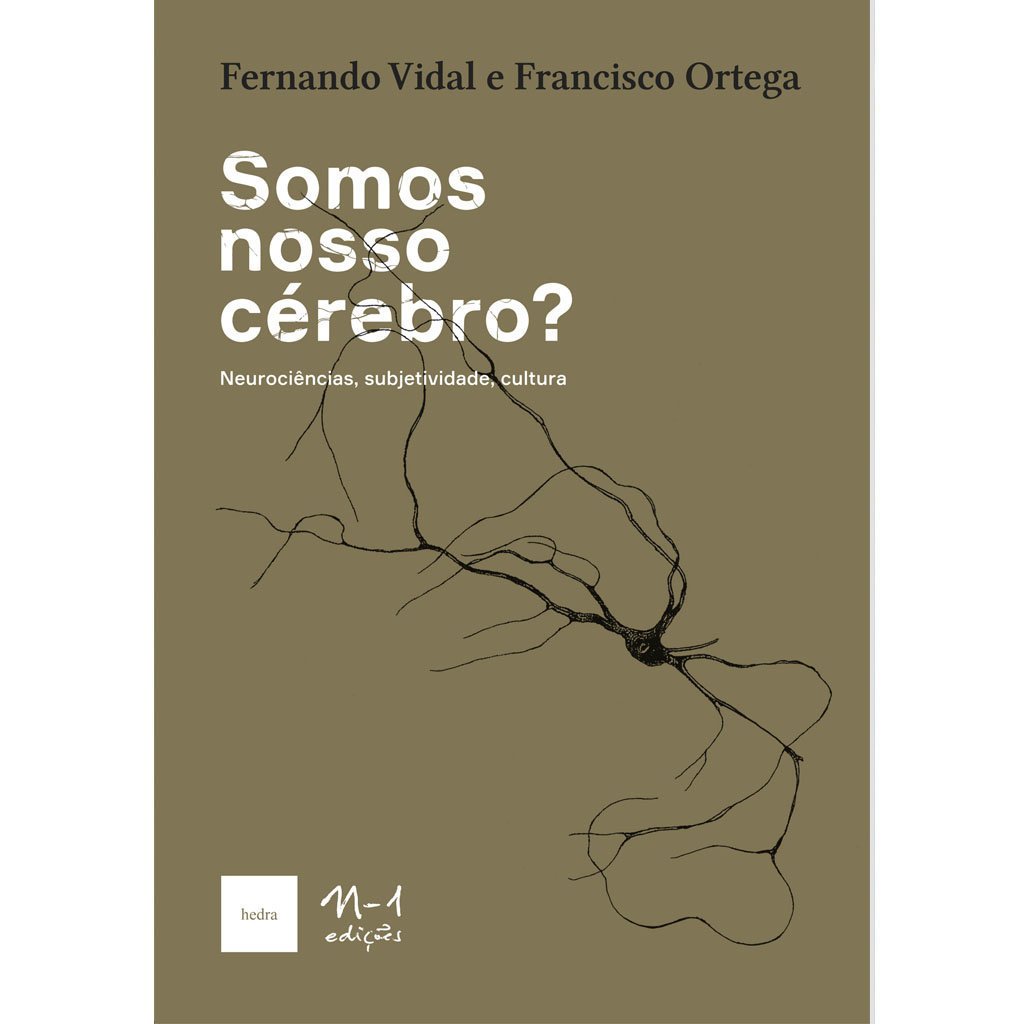
\includegraphics[width=78mm]{./grid/cerebro.png}
\end{center}

\hspace*{-7cm}\hrulefill\hspace*{-7cm}

\medskip

\noindent{}Explorando o neurocentrismo, a crença de que “somos nossos cérebros” se difundiu nos anos 1990. Encorajados pelos avanços da neuroimagem, as humanidades e as ciências sociais adotaram uma “virada neurocientífica” na forma de neuro"-subespecialidades em campos como antropologia, estética, educação, história, direito, sociologia e teologia. Empresas comerciais duvidosas, mas bem"-sucedidas, como “neuromarketing” e “neurobica” surgiram para tirar proveito da sensibilidade aumentada para todo o universo neuro.

Embora não seja hegemônica nem monolítica, a visão neurocêntrica encarna uma poderosa ideologia que está no cerne de alguns dos mais importantes debates filosóficos, éticos, científicos e políticos da atualidade. {\slsc{Somos nosso cérebro?}} escolhido livro do ano em 2018 pela {\slsc{International Society for the History of the Neurosciences}}, examina a lógica interna de tal ideologia, sua genealogia e suas principais encarnações contemporâneas. 


\vfill

\hspace*{-.4cm}\begin{minipage}[c]{.5\linewidth}
\small{
{\Formular{\textbf{
\hspace*{-.1cm}Título: Somos nosso cérebro?\\ Neurociências, subjetividade, cultura\\
Autor: Francisco Ortega e Fernando vidal\\ 
ISBN: 978-65-9582-035-7\\
Páginas: 346\\
Formato: 16x23cm\\
Preço: R\$ 80,00\\
Editora: n-1 \& Hedra\\
Disponibilidade: Disponível
}}}}
\end{minipage}

\pagebreak %PRAGMATISMO PULSIONAL


\begin{center}
\hspace*{-3.5cm}\raisebox{5.4cm}{\rotatebox[origin=t]{90}{\huge\Formular{\textbf{Lançamento}}}}
\hspace*{3cm}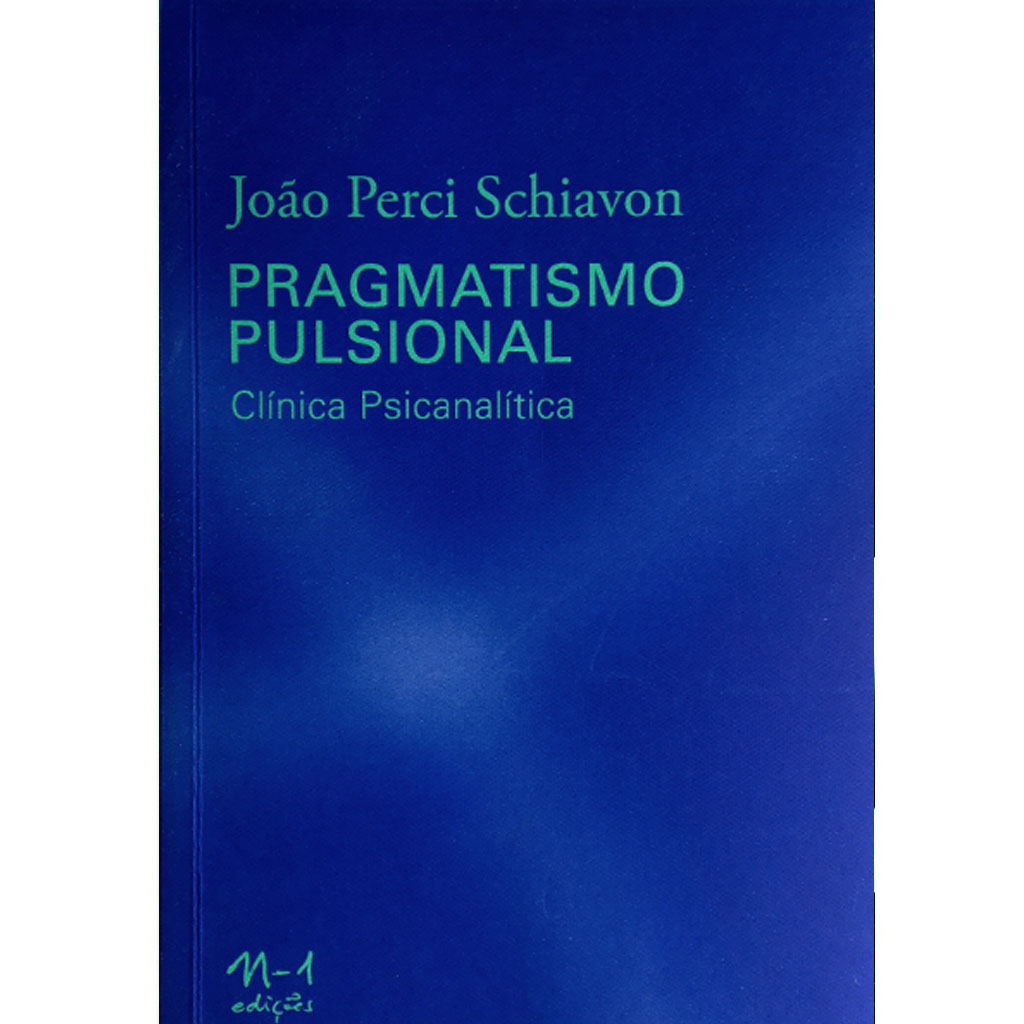
\includegraphics[width=78mm]{./grid/gozo.jpg}
\end{center}

\hspace*{-7cm}\hrulefill\hspace*{-7cm}

\medskip

\noindent{}Raros são os psicanalistas que têm tamanho domínio de Lacan e de Guattari a um só tempo, e que a exemplo de João Perci Schiavon, professor da \scalebox{.8}{PUC-SP} e autor de obras como {\slsc{A lógica da vida desejante}}, conseguem alcance clínico e filosófico de tal envergadura.  

A uma atmosfera de convite a experimentação do fluxo inconsciente e aposta clínica num diapasão em tudo singular entrecruza assuntos --- a contribuição freudiana à linhagem filosófica que vai de Nietzsche a Deleuze. E a pulsão reaparece sob nova luz: o gozo, este que não serve a nenhum bem, engendra todos os bens possíveis e todas as utilidades, algo desconcertante se tivermos em vista o título do escrito, {\slsc{Pragmatismo pulsional}}.

O livro pode ser lido e vivido como “experiência” subjetiva, clínica, filosófica, micropolítica --- isto é, de transformação. O que mais se pode exigir de um livro hoje além de que faça diferença, e diferença para a vida? A pulsão é uma autoridade no que diz respeito ao vivo ou ao desejo. Ela só precisa ser exercida, e o nome desse exercício é cura.

\vfill

\hspace*{-.4cm}\begin{minipage}[c]{.8\linewidth}
\small{
{\Formular{\textbf{
\hspace*{-.1cm}Título: Pragmatismo pulsional – clínica psicanalítica\\
Autor: João Perci Schiavon\\ 
ISBN: 978-65-8109-706-6\\
Páginas: 336\\
Formato: 14x21cm\\
Preço: R\$ 66,00\\
Editora: n-1\\
Disponibilidade: Disponível
}}}}
\end{minipage}

\pagebreak %FASCISMO OU REVOLUÇÃO? MAURICIO LAZZARATO


\begin{center}
\hspace*{.5cm}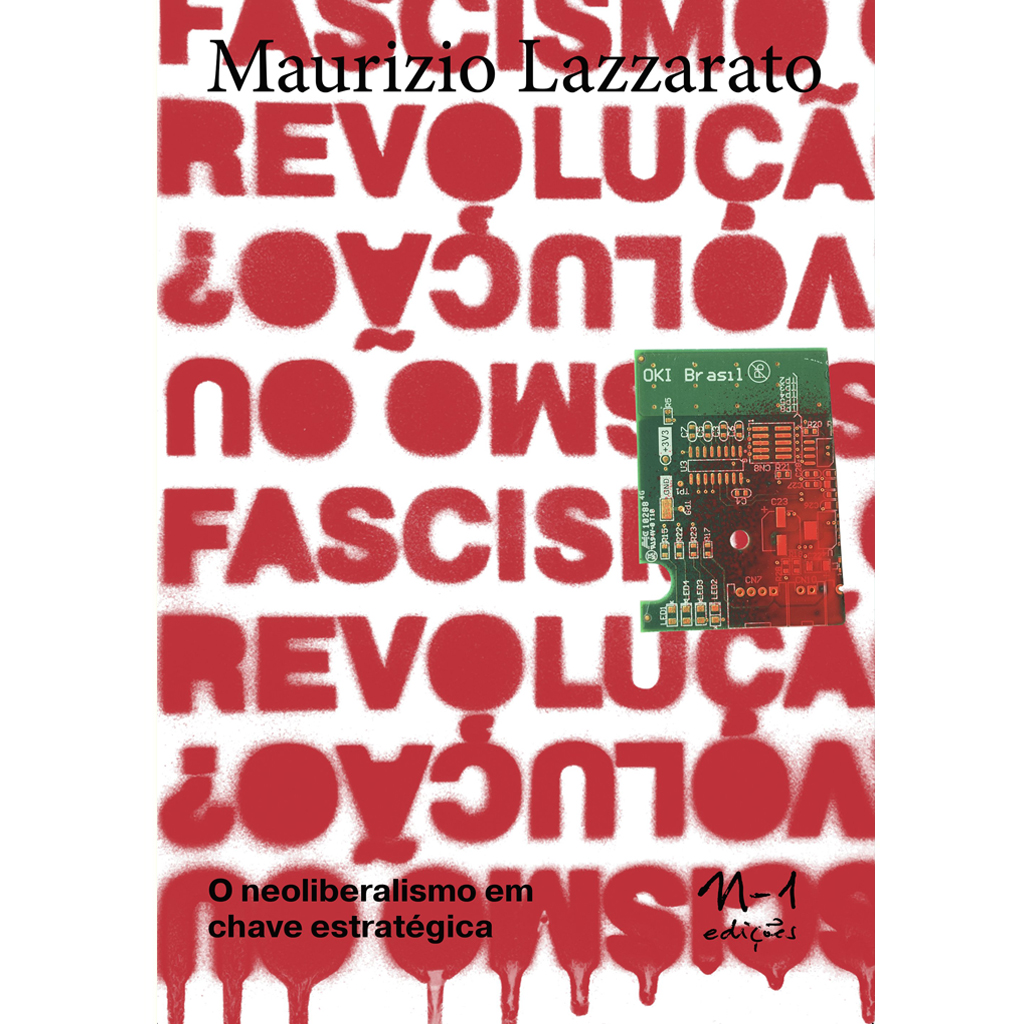
\includegraphics[width=78mm]{./grid/lazzarato.png}
\end{center}

\hspace*{-7cm}\hrulefill\hspace*{-7cm}

\medskip

\noindent{}O fascismo histórico foi tão moderno quanto o capitalismo (já que é uma de suas expressões), como demonstrado nitidamente pelo futurismo italiano. O mesmo ocorre com o novo fascismo, que é um ciberfascismo. Ele põe em xeque todas as utopias tecnociber (do ciberpunk ao ciberfeminismo, da ciberesfera à cibercultura) que desde o pós"-guerra, principalmente a partir dos anos 1970, viam nas máquinas cibernéticas uma dupla promessa: a de uma nova subjetividade pós"-humana e a da liberação da dominação capitalista, cuja ruptura viria das máquinas e não da política. Das revoluções da técnica e não da organização revolucionária.

Bolsonaro e Trump utilizaram todas as tecnologias disponíveis da comunicação digital, mas suas vitórias não vêm da tecnologia. São o resultado da máquina política e estratégia que agencia uma micropolítica dos afetos tristes (frustração, ódio, inveja, angústia medo) com relação à macropolítica de um novo fascismo, que dá consistência política às subjetividades devastadas na financeirização.

\vfill

\hspace*{-.4cm}\begin{minipage}[c]{.5\linewidth}
\small{
{\Formular{\textbf{
\hspace*{-.1cm}Título: Fascimo ou Revolução?\\
Autor: Mauricio Lazzarato\\ 
ISBN: 978-85-6694-381-8\\
Páginas: 208\\
Formato: 14x21cm\\
Preço: R\$ 69,00\\
Editora: n-1\\
Disponibilidade: Disponível
}}}}
\end{minipage}

\pagebreak %ESPAÇO CORUJA

\begin{center}
\hspace*{-3.5cm}\raisebox{5.4cm}{\rotatebox[origin=t]{90}{\huge\Formular{\textbf{Lançamento}}}}
\hspace*{3cm}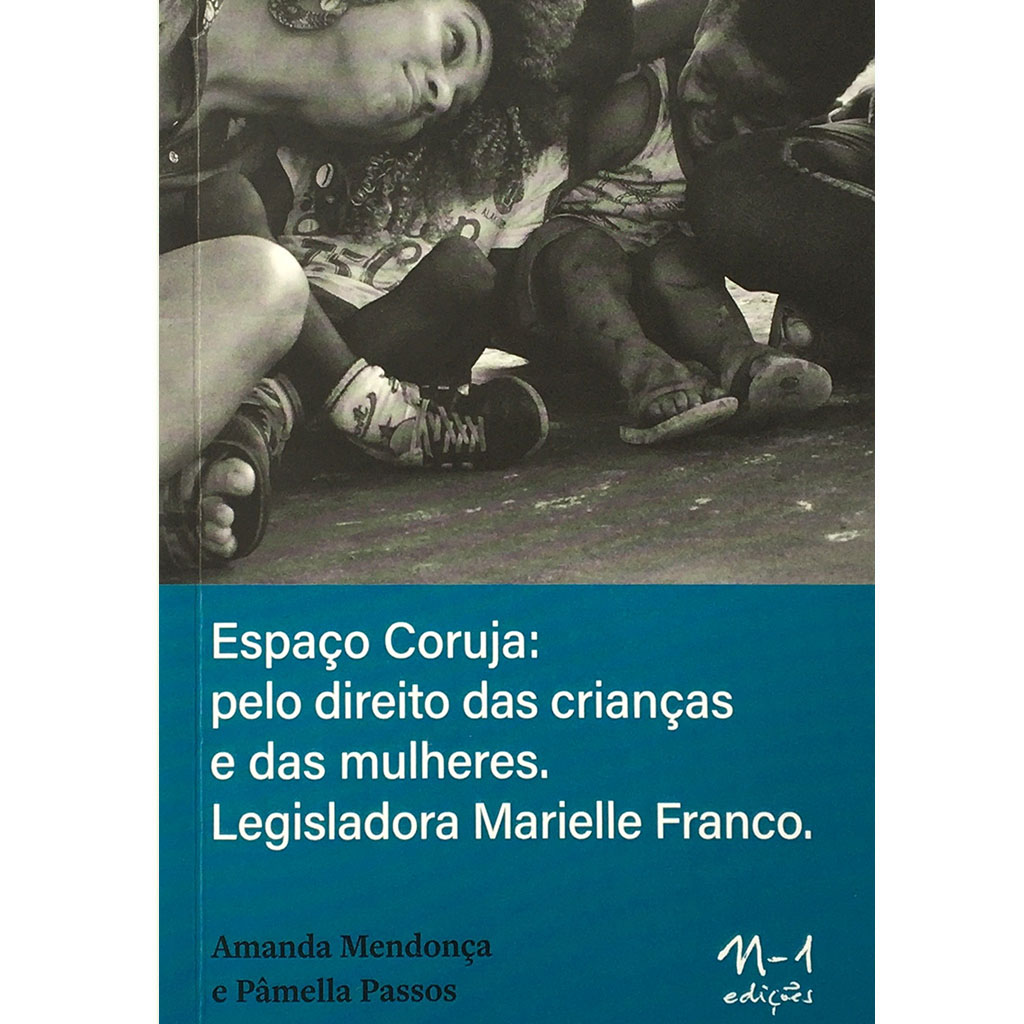
\includegraphics[width=78mm]{./grid/coruja.jpg}
\end{center}

\hspace*{-7cm}\hrulefill\hspace*{-7cm}

\medskip

\noindent{}“A formulação do Projeto de Lei do Espaço Coruja foi uma das ações de maior impacto emocional para Marielle. Era a sua história: uma mulher negra, favelada, que foi mãe jovem e precisava de um lugar seguro para deixar sua filha enquanto trabalhava e estudava. Ela teve uma rede de familiares e de amigos que lhe garantiu avançar e concluir seus estudos. Mas conhecia as diversas e duras realidades da maioria das mulheres que não possuem essa oportunidade. Com empatia e olhar solidário, ela propôs, como legisladora, a criação do Espaço Infantil Noturno. Foram muitos os momentos em que a vi preocupada e empenhada com a elaboração desse projeto tão caro a ela. Ouvinte ativa às críticas, sempre buscou ponderar, mas tinha em seu próprio corpo e história de vida a certeza da urgência. Com essa lei, crianças terão direito a um lugar seguro enquanto suas mães e pais trabalham e/ou estudam --- em um mundo mais justo e igualitário e movimentando as estruturas dessa sociedade ainda tão patriarcal, misógina, machista e racista.” [Mônica Benício]


\vfill

\hspace*{-.4cm}\begin{minipage}[c]{1\linewidth}
\small{
{\Formular{\textbf{
\hspace*{-.1cm}Título: Espaço Coruja: pelo direito das crianças e das mulheres\\
Autor: Amanda Mendonça e Pâmella Passos\\ 
ISBN: 978-65-8109-705-9\\
Páginas: 64\\
Formato: 10x16cm\\
Preço: R\$ 20,00\\
Editora: n-1\\
Disponibilidade: Disponível
}}}}
\end{minipage}

\pagebreak %UM PIANO NAS BARRICADAS, TARÌ

\begin{center}
\hspace*{.5cm}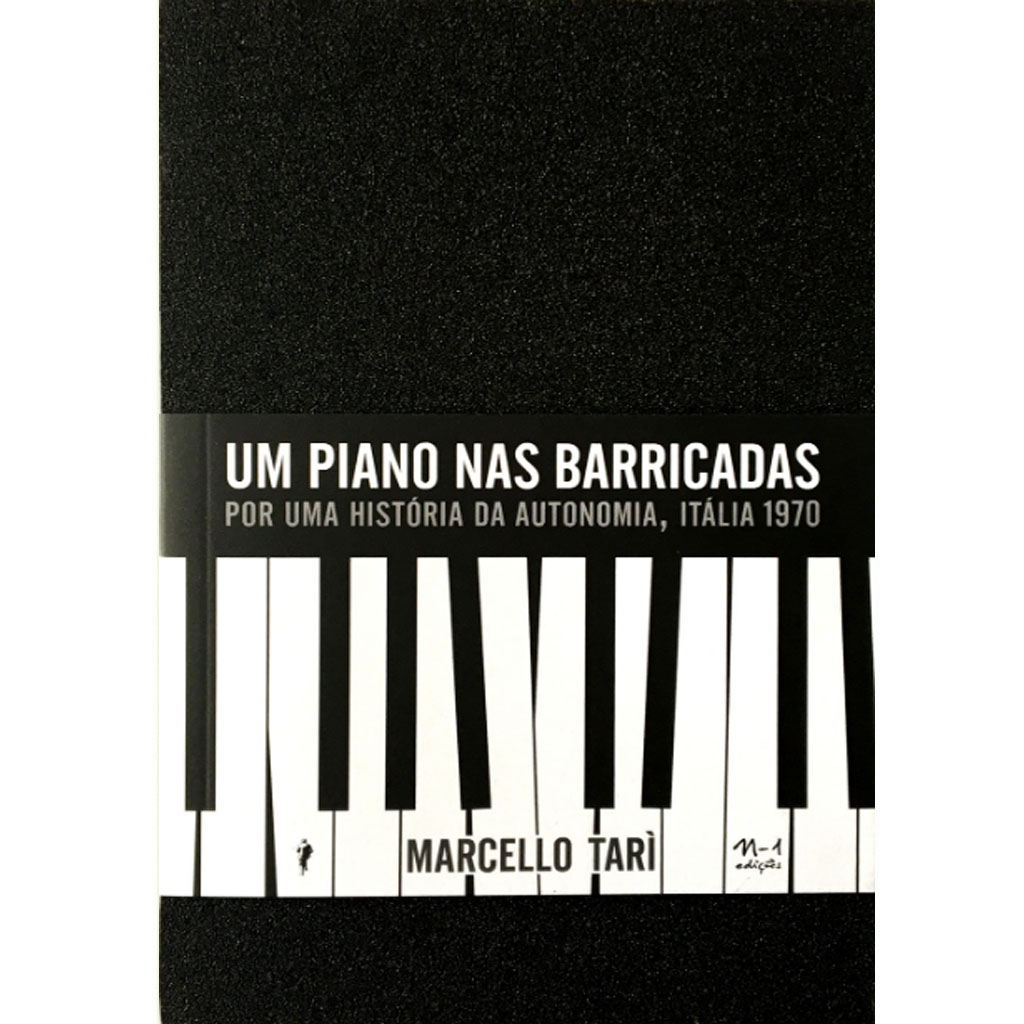
\includegraphics[width=78mm]{./grid/barricada.png}
\end{center}

\hspace*{-7cm}\hrulefill\hspace*{-7cm}

\medskip

\noindent{}Nos filmes sociais e políticos dos anos 1970 na Itália, a Autonomia é apresentada como um método intermediário entre Marx e a antipsiquiatria, a Comuna de Paris e a contracultura, o dadaísmo e o insurrecionalismo, o operaísmo e o feminismo e muitas coisas com outras coisas. Mas apresentou acima de tudo descontinuidade profunda com a prática do Movimento Operário oficial. Não era e nunca foi uma organização, mas uma multiplicidade que se organizava a partir de onde residiam, trabalhavam ou estudavam os sujeitos que a deram forma.

Na Autonomia, muitas autonomias específicas surgiram e coexistiram: operários, estudantes, mulheres, homossexuais, prisioneiros --- ou de qualquer um que escolhesse, a partir de suas próprias contradições, o caminho da luta por um modo reluzente de subversão da vida contra o trabalho assalariado e o Estado. Se o Movimento dos anos 1970 acabou sucumbindo às forças combinadas da máquina estatal e do Partido Comunista, a história da autonomia destaca"-se desse contexto, pois é a de uma aventura revolucionária cuja incandescência atual é mais relevante do que nunca. 

\vfill

\hspace*{-.4cm}\begin{minipage}[c]{1\linewidth}
\small{
{\Formular{\textbf{
\hspace*{-.1cm}Título: Um piano nas barricadas – por uma história da autonomia\\
Autor: Marcelo Tarì\\ 
ISBN: 978-65-8042-104-6\\
Páginas: 384\\
Formato: 12x19cm\\
Preço: R\$ 80,00\\
Editora: n-1 \& Glac\\
Disponibilidade: Disponível
}}}}
\end{minipage}

\pagebreak %FAVARRETO


\begin{center}
\hspace*{-3.5cm}\raisebox{5.4cm}{\rotatebox[origin=t]{90}{\huge\Formular{\textbf{Lançamento}}}}
\hspace*{3cm}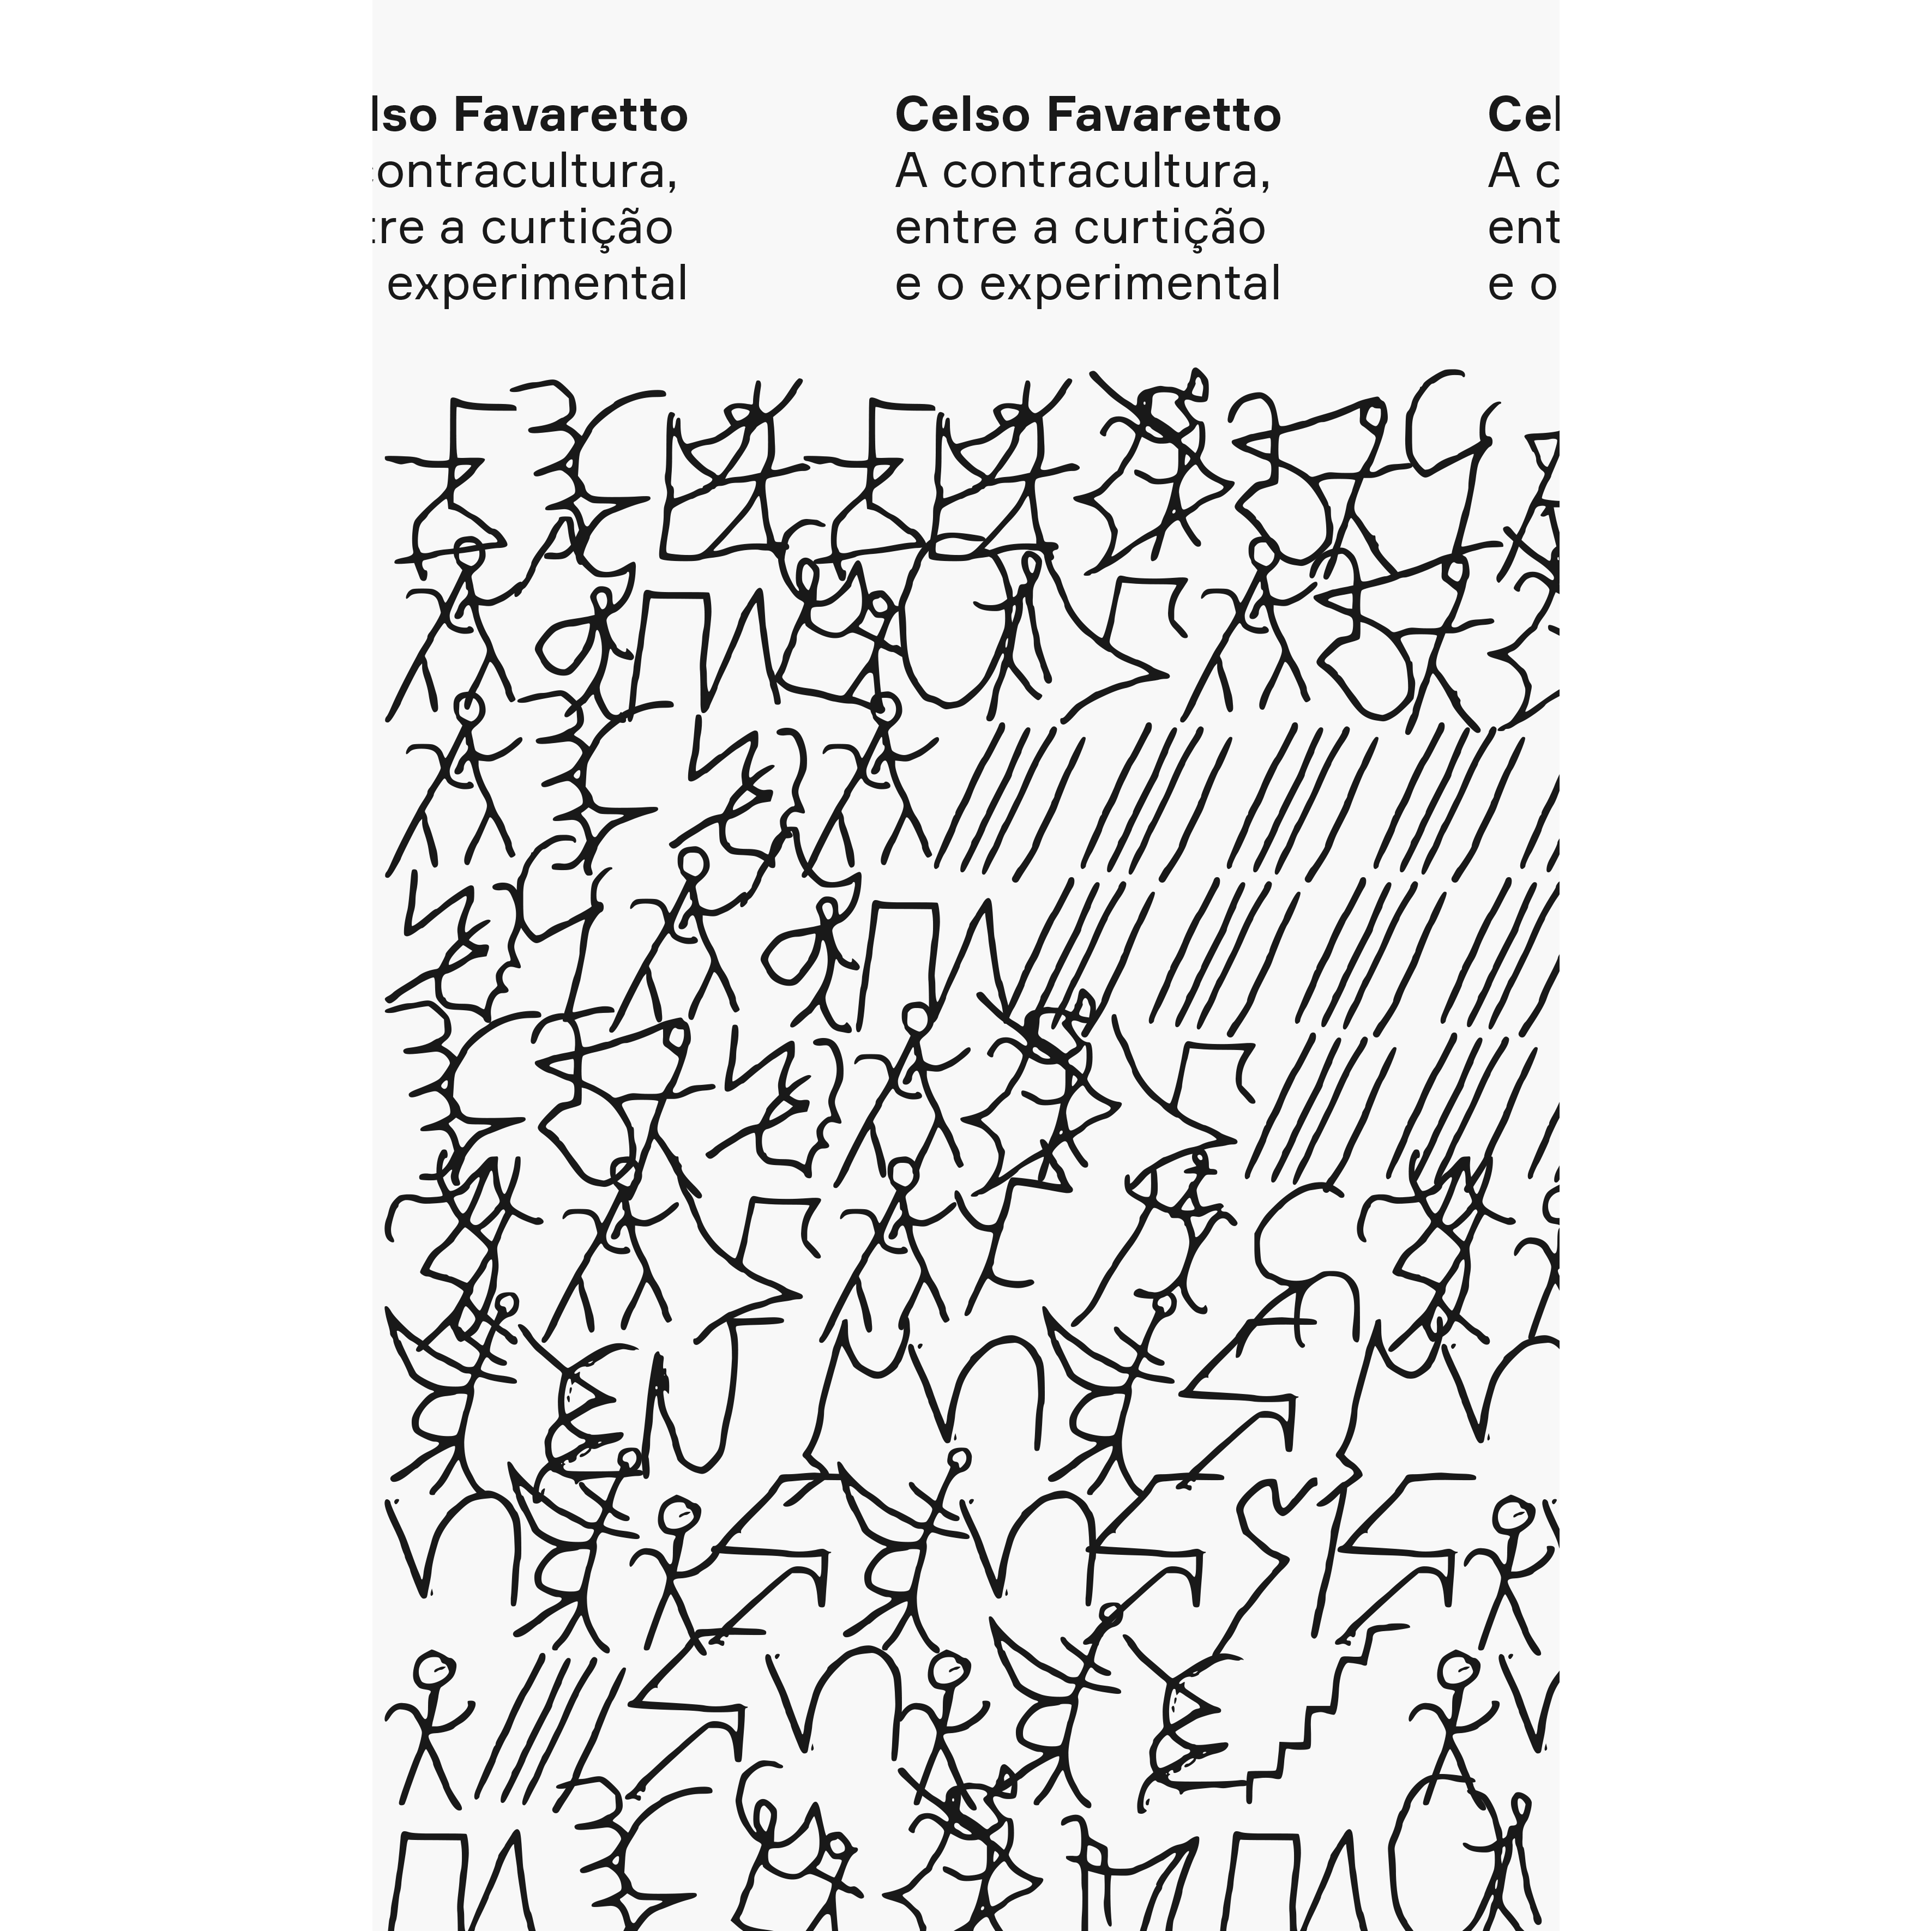
\includegraphics[width=78mm]{./grid/favaretto.png}
\end{center}

\hspace*{-7cm}\hrulefill\hspace*{-7cm}

\medskip

\noindent{}Neste livro o pesquisador e intelectual Celso Favaretto aborda as manifestações contraculturais que marcaram a produção artística brasileira entre os anos 60 e 70. Manifestava"-se então uma nova sensibilidade às margens da política oficial e da indústria cultural, expressa em experimentações artísticas com diversas possibilidades abertas pelo tropicalismo. Longe de um suposto “vazio cultural”, a contracultura nas variadas expressões definiu atitudes, comportamentos, gestos exemplares, experimentações de grande vitalidade. Inclusive, em alguns casos, a resistência às limitações da cultura oficial e à repressão da ditadura.

Composto por três ensaios, são revisitados no livro importantes personalidades e eventos da cultura brasileira --- como Caetano Veloso, Waly Salomão, Glauber Rocha, Zé Celso e o Teatro Oficina, Augusto Boal, Antonio Callado, José Agrippino de Paula, Hélio Oiticica --- sincrônicos aos desdobramentos políticos e sociais implicados pelo Golpe Civil"-Militar.

\vfill

\hspace*{-.4cm}\begin{minipage}[c]{.5\linewidth}
\small{
{\Formular{\textbf{
\hspace*{-.1cm}Título: A contracultura, entre\\ a curtição e o experimental\\
Autor: Celso Favaretto\\ 
ISBN: 978-65-8109-703-5\\
Páginas: 142\\
Formato: 11x18cm\\
Preço: R\$ 40,00\\
Editora: Hedra \& n-1\\
Disponibilidade: Disponível
}}}}
\end{minipage}

\pagebreak %RITORNELOS

\begin{center}
\hspace*{.5cm}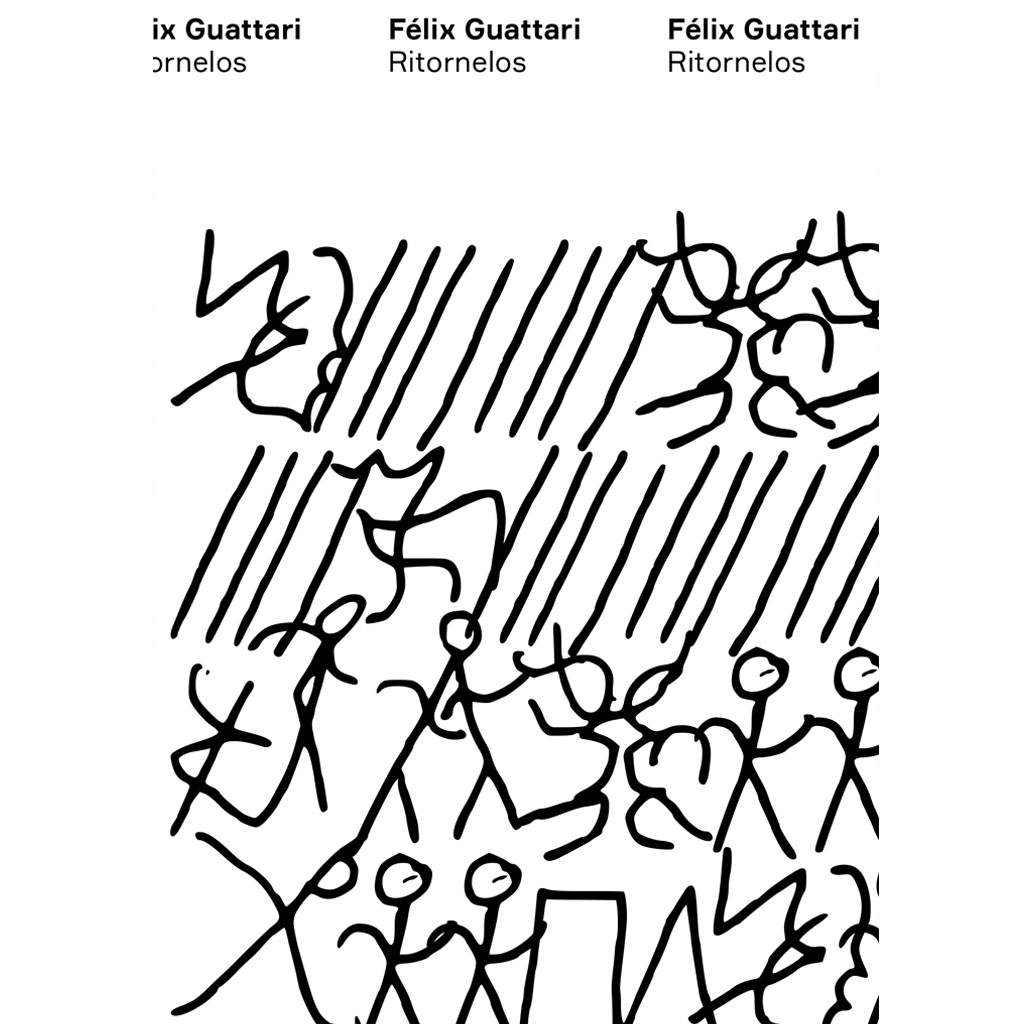
\includegraphics[width=78mm]{./grid/guattari.jpg}
\end{center}

\hspace*{-7cm}\hrulefill\hspace*{-7cm}

\medskip

\noindent{}Livro póstumo do pensador e psicanalista francês Félix Guattari, {\slsc{Ritornelos}} é uma obra inclassificável. Misto de poesia, relatos autobiográficos, {\slsc{frames}} do cotidiano, toda potência da escrita esquiza irrompe nessas páginas de alta voltagem poética e imagética. Além de arguto intelectual, Guattari aparece em {\slsc{Ritornelos}} enquanto poeta sensível aos instantâneos e surreais quadros da vida.

Ao longo de suas páginas, vemos a fluidez com que a escrita de Guattari escorre sobre a superfície da vida, penetra em suas estruturas fragmentadas e as transporta ao seu revés. Através desse torvelinho de imagens decompostas o livro leva o leitor a percorrer o universo único do filósofo: cenas de amor e intimidade, de amizades, captadas nas ruas e praças parisienses, suas referências literárias e cinematográficas, quase em um mapeamento afetivo e cartográfico do autor de {\slsc{O anti-Édipo}}. Publicado somente nos anos 2000 na França, é a primeira vez que o livro é traduzido e editado no Brasil, em trabalho minucioso de tradutor"-ourives para acompanhar todas as nuances, rupturas e labirintos do texto original.

\vfill

\hspace*{-.4cm}\begin{minipage}[c]{.5\linewidth}
\small{
{\Formular{\textbf{
\hspace*{-.1cm}Título: Ritornelos\\
Autor: Félix Guattari\\ 
ISBN: 978-65-8109-702-8\\
Páginas: 134\\
Formato: 11x18cm\\
Preço: R\$ 40,00\\
Editora: Hedra \& n-1\\
Disponibilidade: Disponível
}}}}
\end{minipage}

\pagebreak


\begin{center}
\hspace*{-3.5cm}\raisebox{5.4cm}{\rotatebox[origin=t]{90}{\huge\Formular{\textbf{Lançamento}}}}
\hspace*{3cm}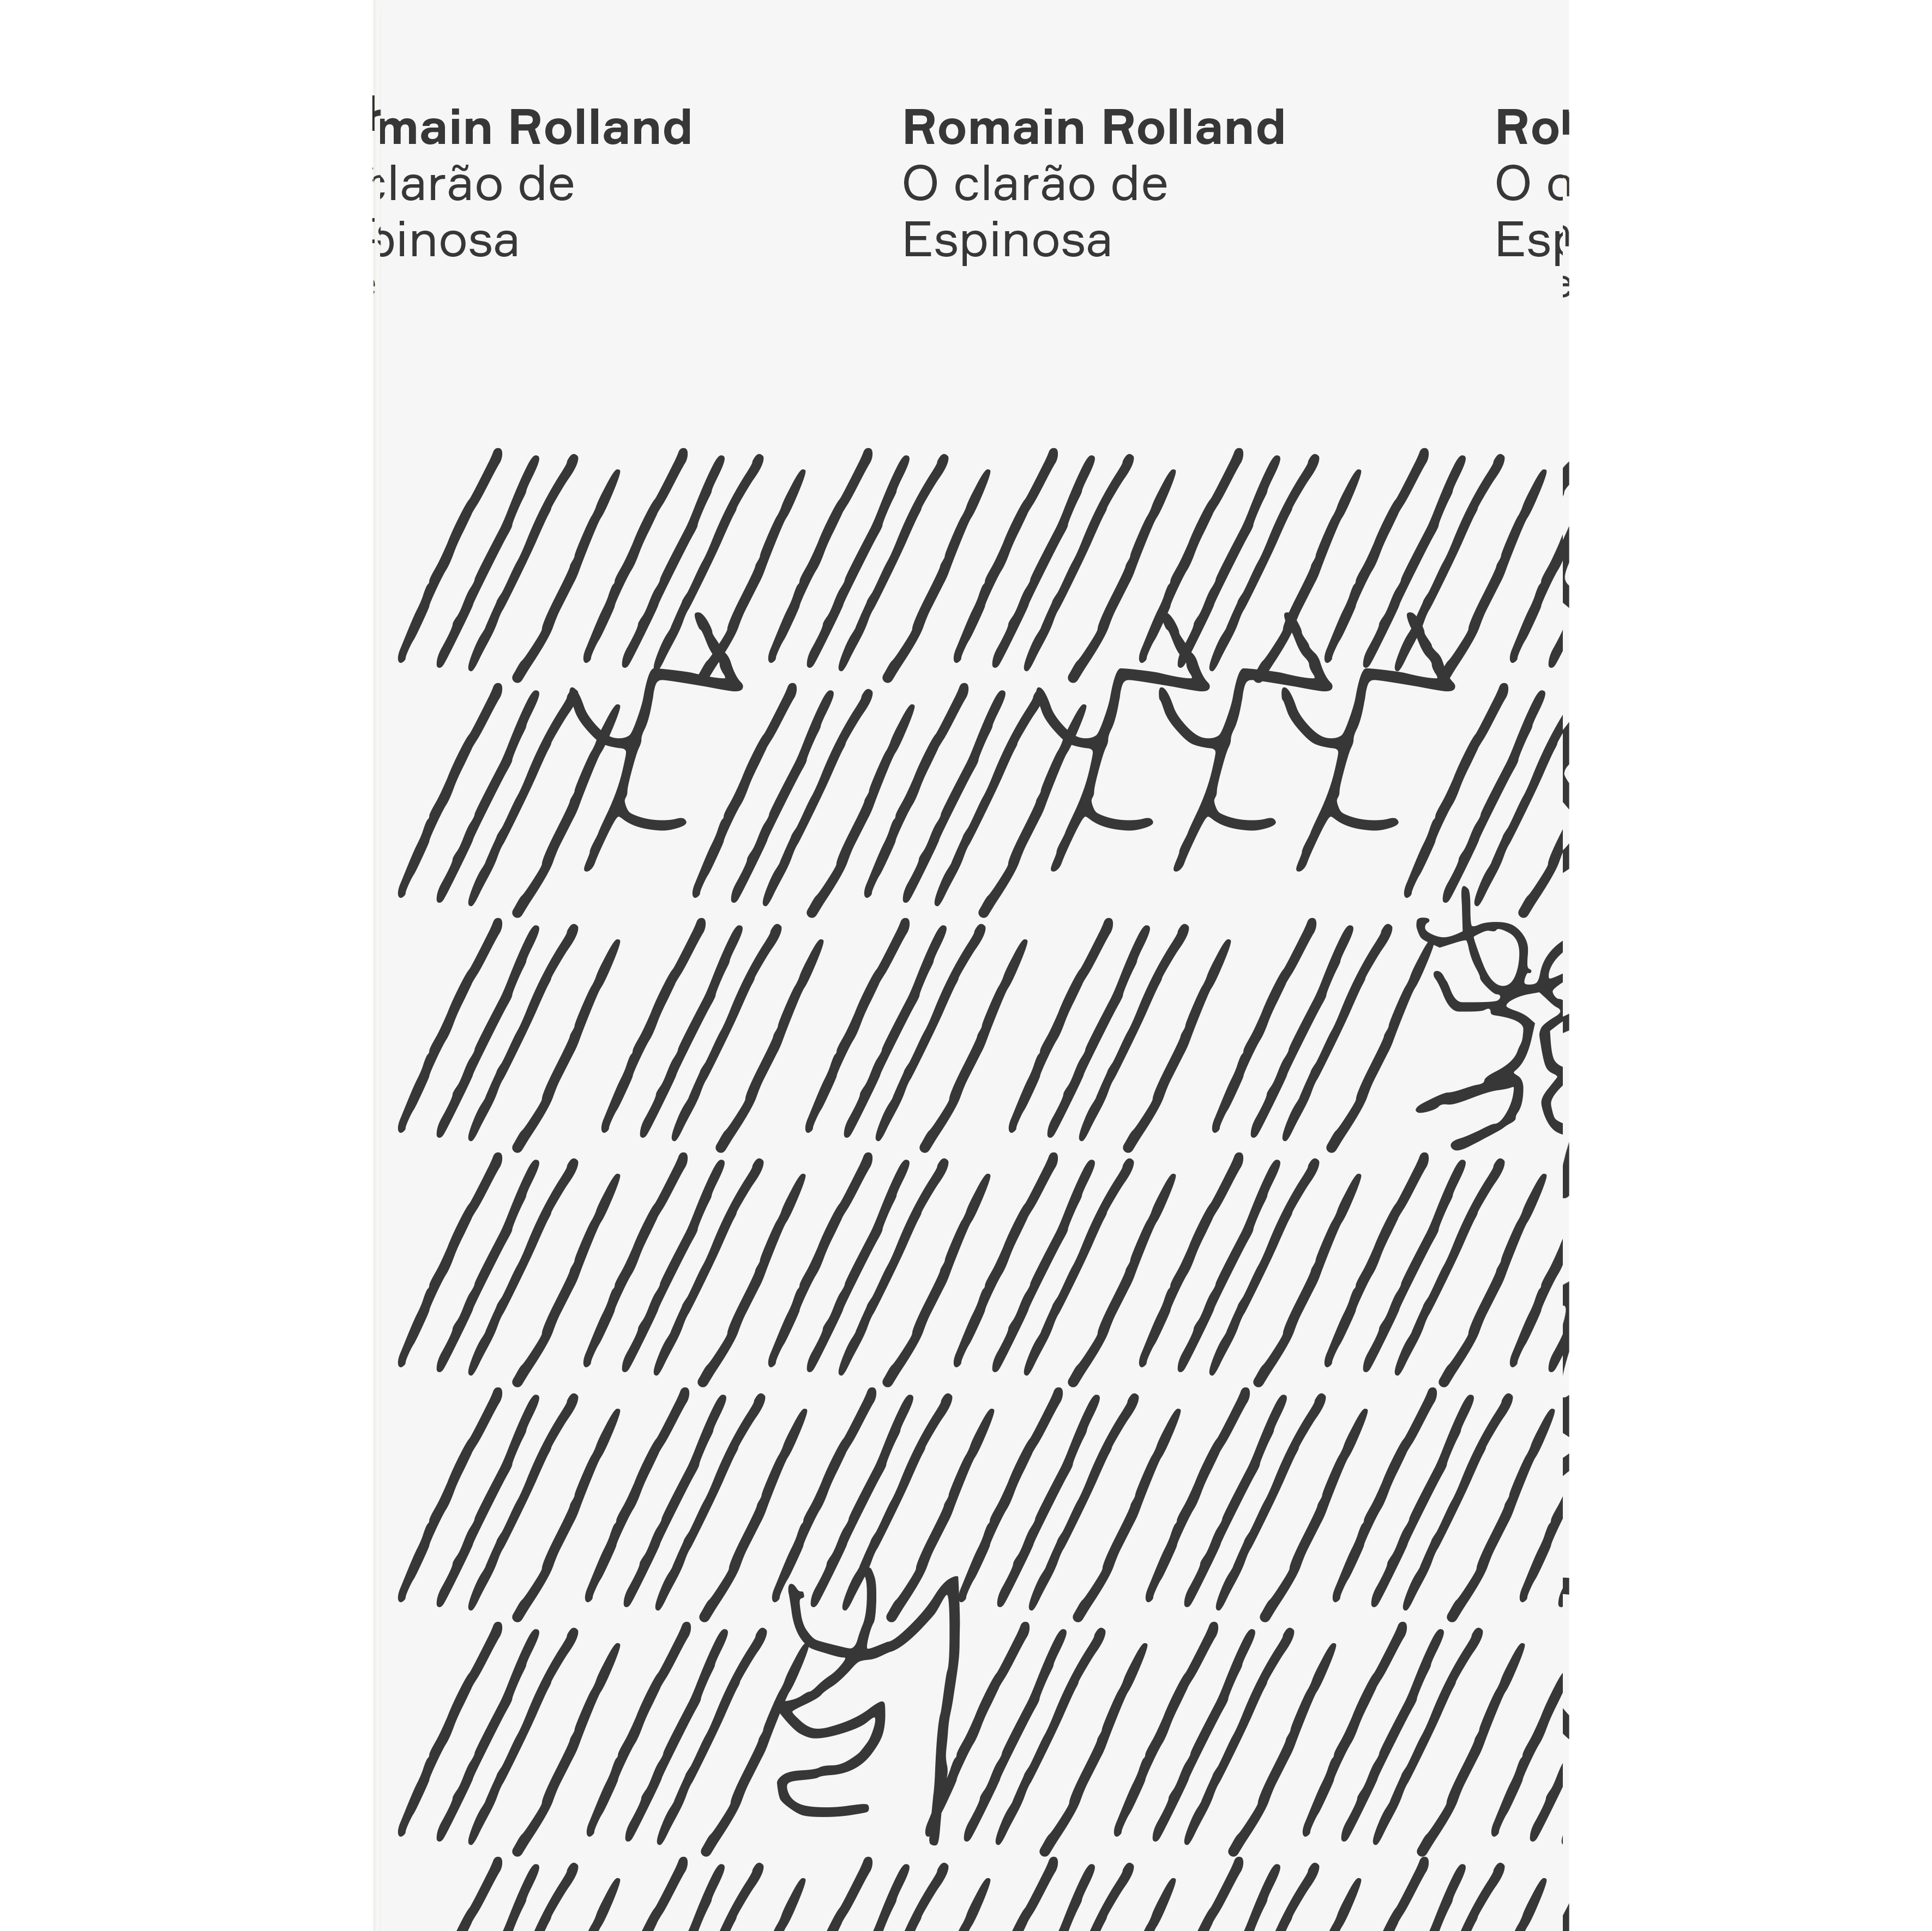
\includegraphics[width=78mm]{./grid/rolland.png}
\end{center}

\hspace*{-7cm}\hrulefill\hspace*{-7cm}

\medskip

\noindent{}Romain Rolland foi novelista, biógrafo, músico e Nobel francês de 1915. Escreveu as presentes páginas sobre Espinosa, repletas de lirismo e potência filosófica, ainda na adolescência, mas foram publicadas apenas em 1942 no livro {\slsc{A viagem interior}}. Neste livro o jovem Rolland conta o “clarão” que teve em sua vida ao ler Espinosa pela primeira vez aos 16 anos, e como isso definiu sua vida e carreira.

Em cuidadosa edição bilíngue, o leitor aproxima"-se dos movimentos luminosos do texto original. O livro é marcado por uma linguagem fremente e impressionista, que segue rente à experiência de deslumbre e atordoamento de Rolland diante da leitura do filósofo. Por trás das imagens poéticas, vislumbra"-se ainda um questionamento existencial e ontológico da condição humana --- reminiscências da filosofia de Espinosa no pensamento e em sua própria prosa. Como escreve o autor, a leitura de Espinosa foi um “desses jatos da alma, desses clarões, que inundaram minhas veias com o fogo que faz bater o coração do universo”. Às “palavras de fogo de Espinosa” dedica"-se esse relato.

\vfill

\hspace*{-.4cm}\begin{minipage}[c]{.5\linewidth}
\small{
{\Formular{\textbf{
\hspace*{-.1cm}Título: O clarão de Espinosa [bilíngue]\\
Autor: Romain Rolland\\ 
ISBN: 978-65-8109-708-0\\
Páginas: 57\\
Formato: 11x18cm\\
Preço: R\$ 29,90\\
Editora: Hedra \& n-1\\
Disponibilidade: 11/09/2020
}}}}
\end{minipage}

\pagebreak

\begin{center}
\hspace*{.5cm}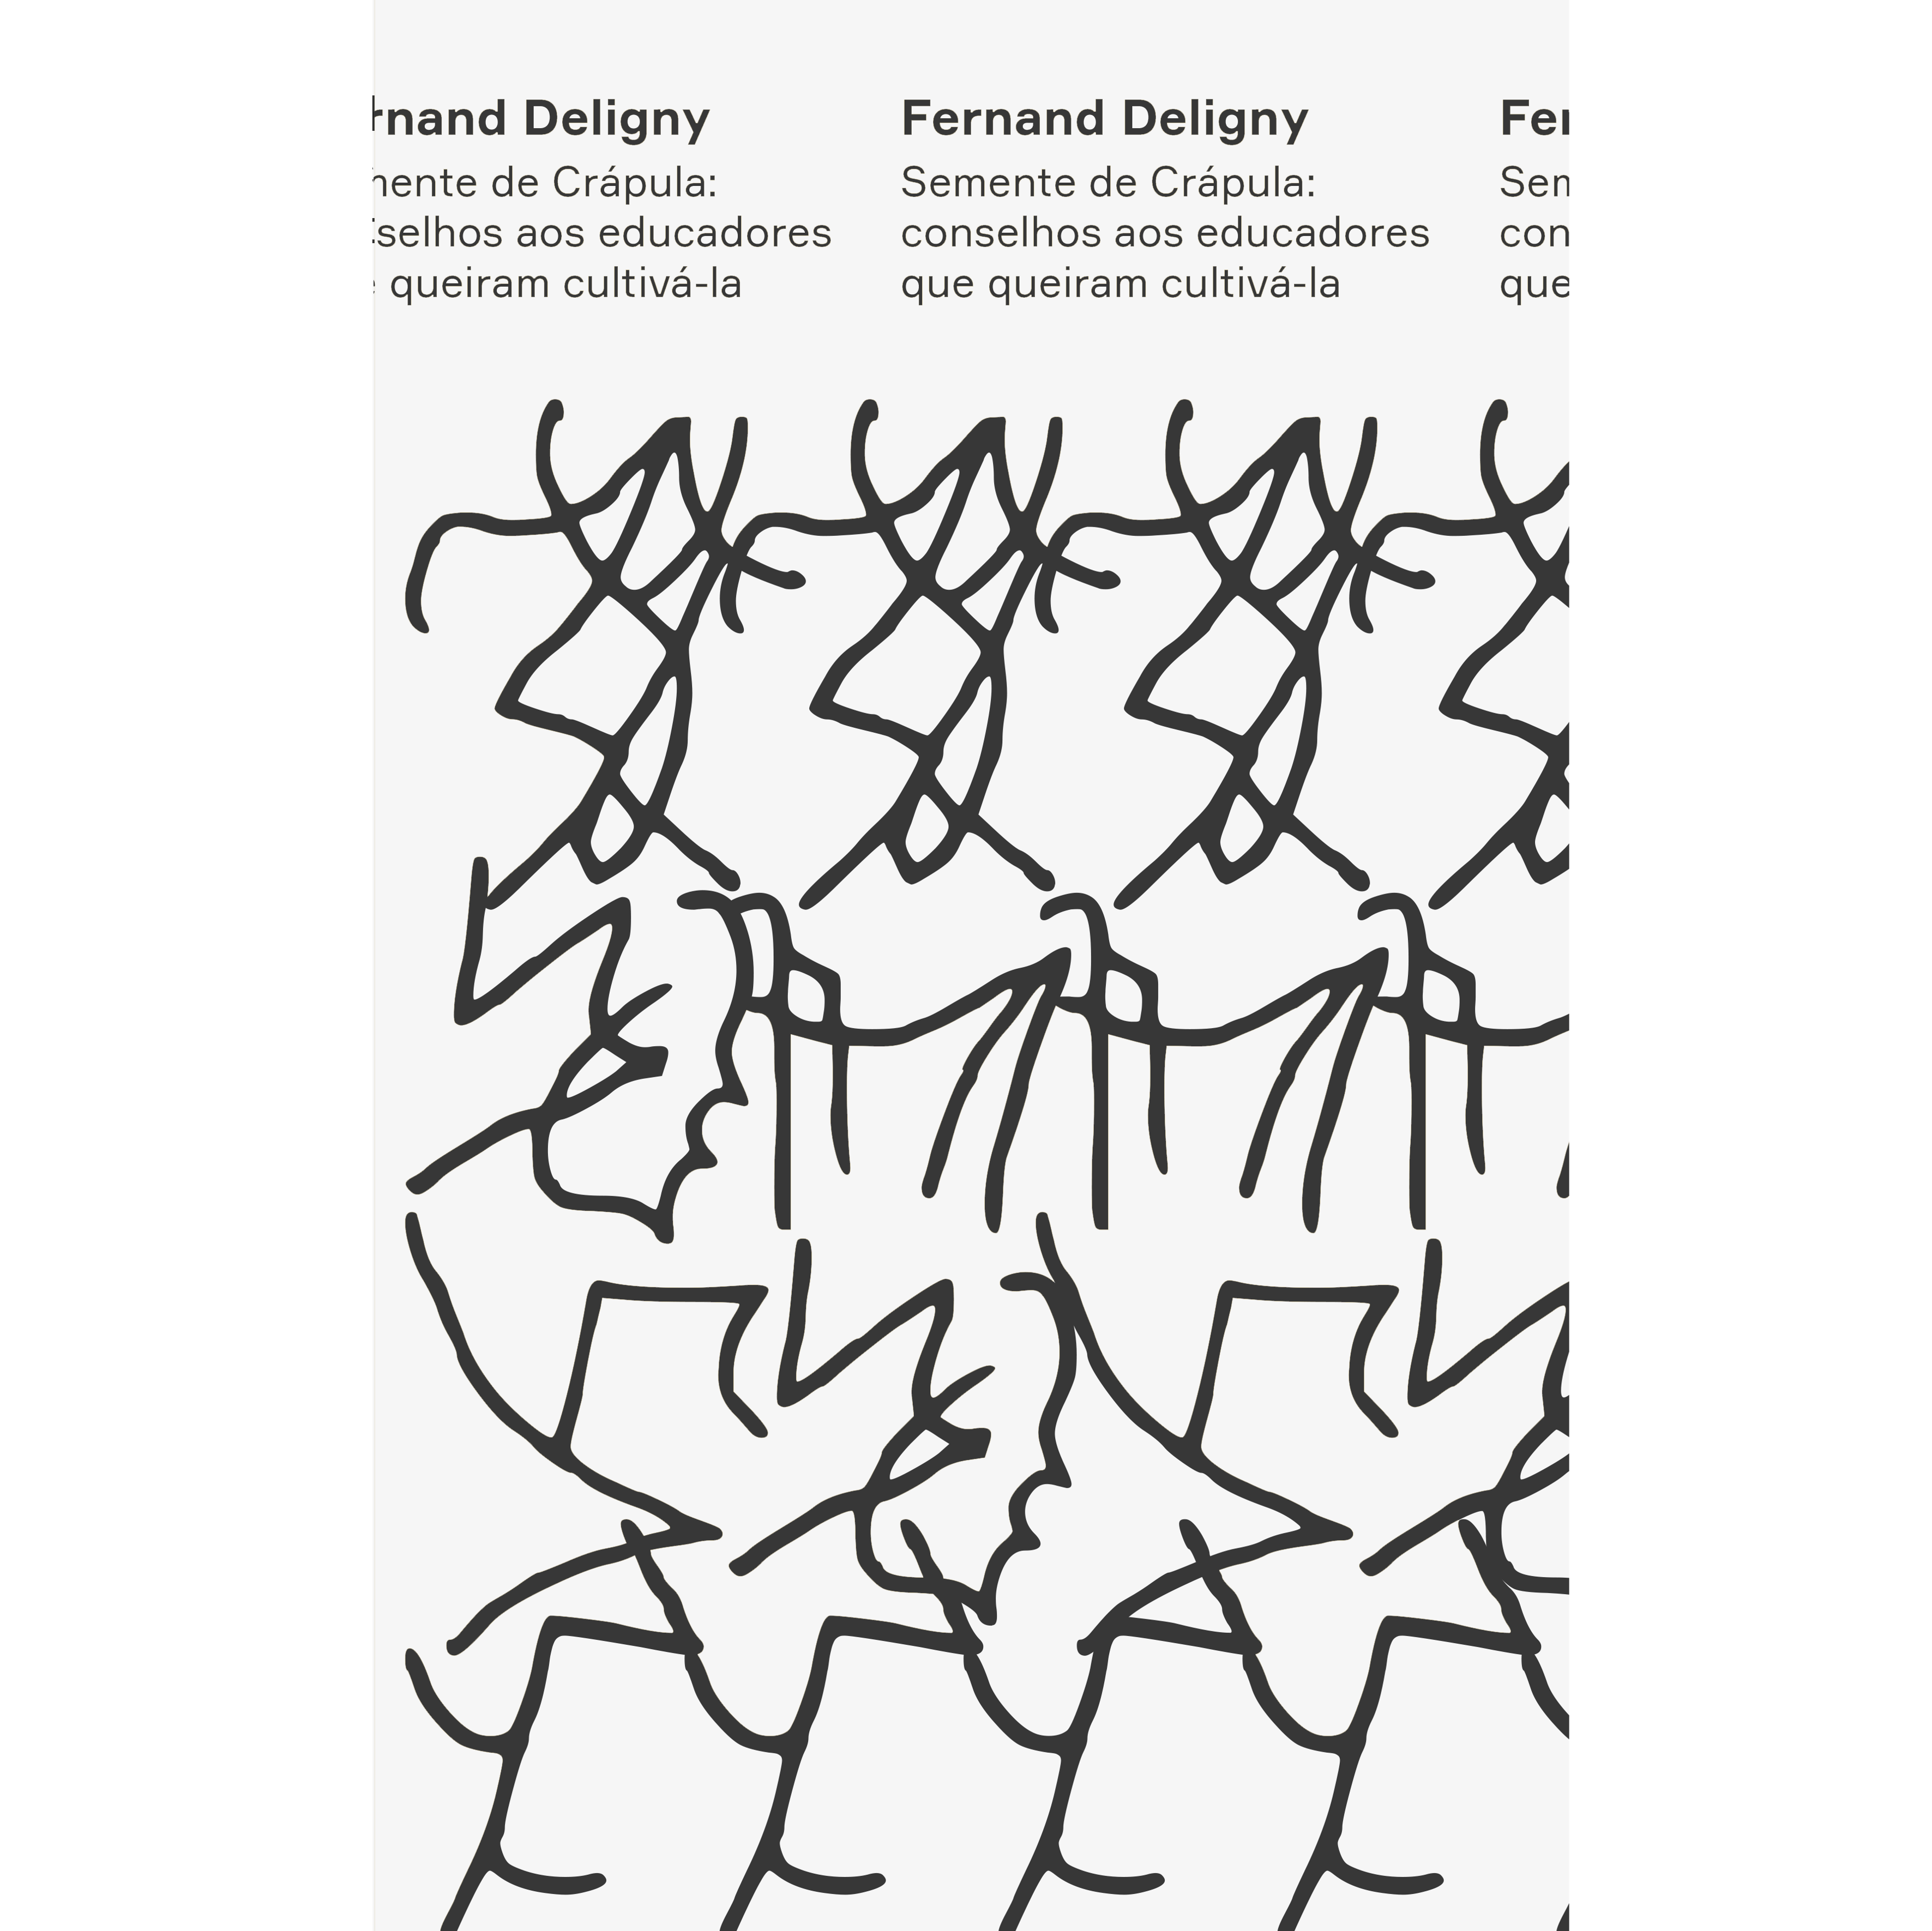
\includegraphics[width=78mm]{./grid/deligny.png}
\end{center}

\hspace*{-7cm}\hrulefill\hspace*{-7cm}

\medskip

\noindent{}{\slsc{Semente de crápula. Conselhos aos educadores que gostariam de cultivá-la}} é o primeiro livro do educador e poeta francês Fernand Deligny. É um balizador de seu trabalho, que o situaria como uma das maiores referências da educação especial --- lidando com crianças e jovens psicóticos, delinquentes, “perigosos”, “marginais” --- e da pedagogia em geral.

Ao longo dos 134 aforismos, Deligny apresenta suas “sementes”: jovens de um meio social delinquente, cultivadas pelo educador que deve deixar de lutar contra as ervas daninhas, pragas sociais atadas ao nosso convívio social, para mergulhar nas dinâmicas espaciais desses jovens que criam outros sentidos de lugar e convivência no território. Publicado em 1945, o livro foi rapidamente bem sucedido na França por sua linguagem poética simples e a franqueza do autor. Deligny passou os primeiros vinte anos de atuação profissional entre escolas especiais, instituições médico"-pedagógicas e hospitais psiquiátricos.

\vfill

\hspace*{-.4cm}\begin{minipage}[c]{1\linewidth}
\small{
{\Formular{\textbf{
\hspace*{-.1cm}Título: Semente de crápula. Conselhos aos educadores que gostariam de cultivá-la\\
Autor: Fernand Deligny\\ 
ISBN: 978-65-8109-709-7\\
Páginas: 96\\
Formato: 11x18cm\\
Preço: R\$ 34,90\\
Editora: Hedra \& n-1\\
Disponibilidade: 11/09/2020
}}}}
\end{minipage}


\pagebreak
\pagestyle{n-1cat}

\begin{multicols}{2}
\begin{enumerate}
\raggedright\nohyphens{
\item Pandemia - Rexistir, {\Formular{\textbf{Eduardo Viveiros de Castro; Achille Mbembe; Carmem Silva; Antonio Negri; Cristina Ribas; Jean Tible; Tatiana Nascimento; Tiqqun; Eduardo Passos; Danichi Hausen Mizoguchi; Yuk Hui}}}
\item Potências do tempo, {\Formular{\textbf{David Lapoujade}}}
\item Declaração, {\Formular{\textbf{Antonio Negri; Michael Hardt}}}
\item Manifesto contrassexual, {\Formular{\textbf{Beatriz Preciado}}}
\item O aracniano e outros textos, {\Formular{\textbf{Fernand Deligny}}}
\item Deleuze, os movimentos aberrantes, {\Formular{\textbf{David Lapoujade}}}
\item Aos nossos amigos, {\Formular{\textbf{Comitê Invisível}}}
\item Teoria King Kong, {\Formular{\textbf{Virginie Despentes}}}
\item Guattari, {\Formular{\textbf{Kuniichi Uno; Laymert Garcia dos Santos}}}
\item Quando e como eu li Foucault, {\Formular{\textbf{Antonio Negri}}}
\item O avesso do niilismo, {\Formular{\textbf{Peter Pál Pelbart}}}
\item A missão, {\Formular{\textbf{Heiner Müller}}}
\item William James, a construção da experiência, {\Formular{\textbf{David Lapoujade}}}
\item Nietzsche - O bufão dos deuses, {\Formular{\textbf{Maria Cristina Franco Ferraz}}}
\item Impressões de Michel Foucault, {\Formular{\textbf{Roberto Machado}}}
\item Fabulações do corpo japonês, {\Formular{\textbf{Christine Greiner}}}
\item As existências mínimas, {\Formular{\textbf{David Lapoujade}}}
\item Hegel e o Haiti, {\Formular{\textbf{Susan Buck-Morss}}}
\item Brazuca, negão e sebento, {\Formular{\textbf{Jean-Christophe Goddard}}}
\item Motim e destituição agora, {\Formular{\textbf{Comitê Invisível}}}
\item Crítica da razão negra, {\Formular{\textbf{Achille Mbembe}}}
\item Testo junkie, {\Formular{\textbf{Paul B. Preciado}}}
\item O universo inacabado, {\Formular{\textbf{Mario Novello}}}
\item Cartas e outros textos, {\Formular{\textbf{Gilles Deleuze}}}
\item Nietzsche e a filosofia, {\Formular{\textbf{Gilles Deleuze}}}
\item Hijikata tatsumi, {\Formular{\textbf{Kuniichi Uno}}}
\item Spartakus, {\Formular{\textbf{Furio Jesi}}}
\item Agamben, {\Formular{\textbf{Giacoia Jr., Oswaldo}}}
\item UPP - A redução da favela em três letras, {\Formular{\textbf{Marielle Franco}}}
\item Cinco dias em março, {\Formular{\textbf{Toshiki Okada}}}
\item Os vagabundos eficazes, {\Formular{\textbf{Fernand Deligny}}}
\item O enigma da revolta, {\Formular{\textbf{Michel Foucault}}}
\item Arqueofeminismo
\item Contribuição para a guerra em curso, {\Formular{\textbf{Tiqqun}}}
\item Ética bixa, {\Formular{\textbf{Paco Vidarte}}}
\item Ensaios do assombro, {\Formular{\textbf{Peter Pál Pelbart}}}
\item Metafísicas canibais, {\Formular{\textbf{Eduardo Viveiros de Castro}}}
\item O governo do homem endividado, {\Formular{\textbf{Maurizio Lazzarato}}}
\item Leituras do corpo no Japão, {\Formular{\textbf{Christine Greiner}}}
\item Pragmatismo pulsional, {\Formular{\textbf{João Perci Schiavon}}}
\item Ruptura, {\Formular{\textbf{Centelha}}}
\item Às voltas com Lautréamont, {\Formular{\textbf{Laymert Garcia dos Santos}}}
\item Afrotopia, {\Formular{\textbf{Felwine Sarr}}}
\item Fascismo ou revolução?, {\Formular{\textbf{Maurizio Lazzarato}}}
\item Corpos que importam, {\Formular{\textbf{Judith Butler}}}
\item Somos nosso cérebro?, {\Formular{\textbf{Francisco Ortega; Fernando Vidal}}}
\item Ritornelos, {\Formular{\textbf{Félix Guattari}}}
\item Contracultura, entre a curtição e o experimental, {\Formular{\textbf{Celso Favaretto}}}
}
\end{enumerate}
\end{multicols}

\pagebreak